\documentclass[11pt, aspectratio=169]{beamer}

% --- Ngôn ngữ và Font ---
\usepackage[utf8]{inputenc}
\usepackage[vietnamese]{babel}
\usepackage[T1]{fontenc}
\usepackage{helvet} % Font không chân hiện đại giống mẫu
\usepackage{tikz}
\usepackage{graphicx}
\usepackage{booktabs}
\usepackage{amsmath}

% --- Giao diện và Màu sắc ---
\usetheme{default}
\usecolortheme{whale}

\definecolor{MainNavy}{RGB}{0, 51, 102} % Màu xanh đậm tiêu đề
\definecolor{MainGold}{RGB}{184, 152, 75}
\definecolor{SubGray}{RGB}{128, 128, 128} % Màu xám phụ đề

\setbeamercolor{title}{fg=MainNavy}
\setbeamercolor{subtitle}{fg=SubGray}
\setbeamercolor{author}{fg=black}
\setbeamercolor{institute}{fg=black}
\setbeamercolor{frametitle}{bg=MainNavy, fg=white}

% --- Loại bỏ các thành phần thừa ---
\setbeamertemplate{navigation symbols}{} % Ẩn các icon điều hướng

% --- Tùy chỉnh trang tiêu đề (Title Page) ---
\setbeamertemplate{title page}{
    \begin{center}
        % Logo hàng đầu
        \begin{figure}[H]
            \centering
            \begin{minipage}{0.3\textwidth}
                \centering
                
\includegraphics[width=0.8\textwidth]{figures/logo-INSA.png}
            \end{minipage}
            \hfill
            \begin{minipage}{0.3\textwidth}
                \centering
                % Thay 'logo-torus' bằng tên file logo công ty bạn
                
\includegraphics[width=0.5\textwidth]{figures/logo-torus.png} 
            \end{minipage}
            \hfill
            \begin{minipage}{0.3\textwidth}
                \centering
                
\includegraphics[width=0.8\textwidth]{figures/logo-N7.png}
            \end{minipage}
        \end{figure}
        
        \vspace{0.5cm}
        
        % Phụ đề
        {\large\color{SubGray} \insertsubtitle}
        \vspace{0.4cm}

        % Tiêu đề chính
        {\Large\bfseries\color{MainNavy} \inserttitle}

        \vfill
        
        % Chia 2 cột cho thông tin học viên và người hướng dẫn
        \begin{columns}[t] % [t] để căn lề trên của 2 cột bằng nhau
            \hfill
            \begin{column}{0.5\textwidth}
                \small
                \textbf{Author:} Minh Duy Nguyen \\
                \textbf{Major:} Mathematical Modeling \& AI \\
                \textbf{Supervisor:} Milad Mozafari (Torus AI) \\
                \textbf{Defense Date:} 05/02/2026
            \end{column}
            
            % Thanh gạch dọc ở giữa
            \vrule{} 
            \hfill
            
            \begin{column}{0.3\textwidth}
               \small
                \textbf{Jury} \\
                David Bertoin \\
                Charles Dossal \\
                Olivier Roustant
            \end{column}
            \hfill
        \end{columns}
    \end{center}
}

% --- Thông tin tài liệu ---
\title{Optimizing and Adapting Language Models for Domain-Specific Task}
\subtitle{End-of-studies Apprenticeship Report}
\author{Minh Duy Nguyen - Báo cáo Thực tập Tốt nghiệp (Master's Report)}
\institute{Milad Mozafari (Torus AI) \& David Bertoin (INSA Toulouse)}
\date{}

\begin{document}

% Slide tiêu đề
\begin{frame}[plain]
    \titlepage
\end{frame}

\begin{frame}{From research to practice: challenges of AI implementation in business}
    95\% AI generation/LLM project in companies fail to generate significant P\&L value. \cite{tomshardware2024mit}\\
    2 challenges in domain-specific NLP tasks:
    - Knowledge Gap
    - Behavior Gap
\end{frame}

\begin{frame}{}
    
\end{frame}



% Slide nội dung mẫu
\begin{frame}{Agenda}
    \begin{itemize}
        \item 
        \item 
        \item 
        \item 
        \item 
    \end{itemize}
\end{frame}

\begin{frame}{The real challenge: Complex financial and healthcare data}
    \begin{columns}[t] % [t] để căn lề trên của 2 cột bằng nhau
        % Cột 1: Tài chính
        \begin{column}{0.48\textwidth}
            \textbf{\color{MainNavy} Case Study 1: Financial}
            \vspace{0.2cm}
            
            \small SFCR report with complex financial tables and charts.
            
            \vspace{0.4cm}
            \centering
            \fbox{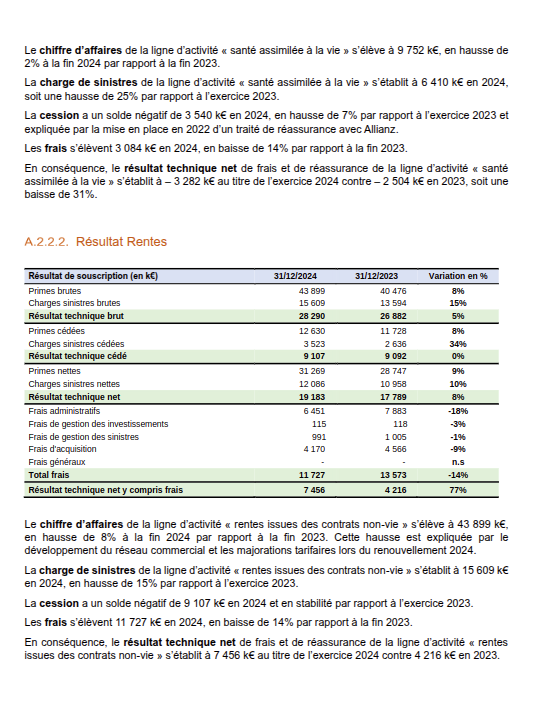
\includegraphics[width=\textwidth]{figures/gpm_report_example.png}} 
            % Note: fbox (if using tcolorbox package) or custom border if needed
        \end{column}

        % Cột 2: Y tế
        \begin{column}{0.48\textwidth}
            \textbf{\color{MainNavy} Case Study 2: Healthcare}
            \vspace{0.2cm}
            
            \small CCAM catalog with thousands of codes requiring exact matching.
            
            \vspace{0.4cm}
            \centering
            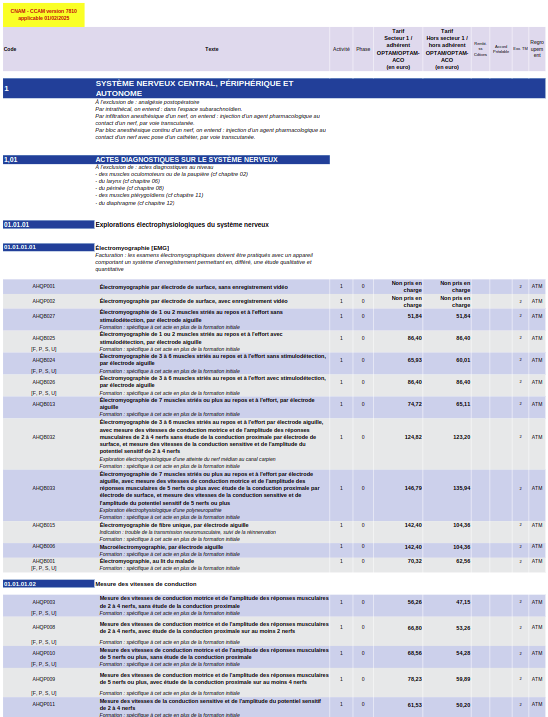
\includegraphics[width=\textwidth]{figures/ccam_example.png}
        \end{column}
    \end{columns}
\end{frame}

\begin{frame}[fragile]{Why SimpleRAG fails: An empirical analysis}
    \small
    % --- Failure 1 ---
    \textbf{\color{MainNavy}Failure 1: Loss of Table Structure}
    \hfill \textit{Extraction using PyPDF}

    \begin{columns}[T]
        \begin{column}{0.45\textwidth}
            \centering
            \resizebox{\linewidth}{!}{
            \begin{tabular}{|l|r|r|r|}
                \hline
                \textbf{Sous modules (en k€)} & \textbf{SCR 2024} & \textbf{SCR 2023} & \textbf{Evol.} \\ % Viết tắt Evolution để đỡ bị tràn
                \hline
                Type 1 & 2 692 & 2 487 & 8 \% \\
                \hline
                Type 2 & 28 377 & 36 221 & -22 \% \\
                \hline
                Diversification & -621 & -586 & 6 \% \\ % Rút gọn text một chút cho đẹp bảng nhỏ
                \hline
                \textbf{Risque de défaut} & \textbf{30 448} & \textbf{38 121} & \textbf{-20 \%} \\
                \hline
            \end{tabular}
        }
        \end{column}
        
        \begin{column}{0.05\textwidth}
            \vspace{0.5cm} $\rightarrow$
        \end{column}
        
        \begin{column}{0.5\textwidth}
            \begin{minipage}[t]{0.48\textwidth}
        \scriptsize 
        \begin{verbatim}
Sous modules (en k€) SCR 2024 SCR 2023 Evolution 
Type 1 2 692 2 487 8 % 
Type 2 28 377 36 221 -22 % 
Effet de diversification -621 -586 6 % 
Risque de défaut 30 448 38 121 -20 %
        \end{verbatim}
    \end{minipage}
            % \tiny \color{navyblue} PyPDF làm phẳng bảng 2 chiều $\rightarrow$ Mất ngữ cảnh hàng/cột.
        \end{column}
    \end{columns}
\end{frame}

\begin{frame}{Why SimpleRAG fails: An empirical analysis}
    \textbf{\color{MainNavy}Failure 2: Failure with exact code matching}
    \hfill \textit{Extraction using PyPDF}

    \begin{columns}[T]
        \begin{column}{0.45\textwidth}
            \centering
            
\includegraphics[width=\textwidth]{figures/search_HAFA.png}
        \end{column}
        
        \begin{column}{0.05\textwidth}
            \vspace{0.5cm} $\rightarrow$
        \end{column}
        
        \begin{column}{0.5\textwidth}
            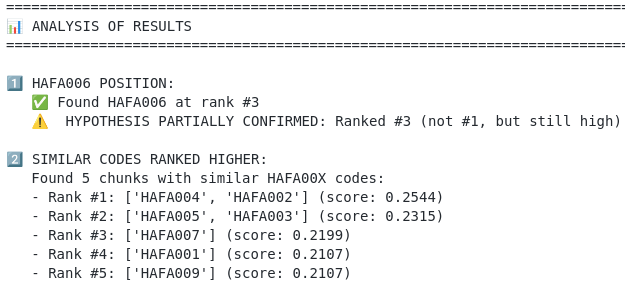
\includegraphics[width=\textwidth]{figures/ccam_dense_search_failure.png}
            % \tiny \color{navyblue} PyPDF làm phẳng bảng 2 chiều $\rightarrow$ Mất ngữ cảnh hàng/cột.
        \end{column}
    \end{columns}
\end{frame}

\begin{frame}{Advanced Multimodal RAG Pipeline}
    \begin{figure}
        \centering
        \includegraphics[width=0.35\textwidth]{figures/rag_pipeline_diagram.png}
    \end{figure}
\end{frame}

\begin{frame}{Experimental Results: Superior accuracy improvement}
    \begin{table}[H]
        \centering
        \caption{Results on GPM Test Set (25 questions)}
        \begin{tabular}{|l|c|c|c|c|}
            \hline
            \textbf{Pipeline} & \textbf{Correctness} & \textbf{Relevancy} & \textbf{Faithfulness} & \textbf{Context Precision} \\
            \hline
            Simple RAG & 0.648 & 0.788 & 0.732 & 0.654 \\
            \hline
            Advanced RAG & \textbf{0.976} & \textbf{0.972} & \textbf{0.94} & \textbf{0.96} \\
            \hline
            \textit{Improvement} & \textit{+32.8\%} & \textit{+18.4\%} & \textit{+20.8\%} & \textit{+30.6\%} \\
            \hline
        \end{tabular}
    \end{table}

    \begin{table}[H]
        \centering
        \caption{Results on CCAM Test Set (10 scenarios)}
        \begin{tabular}{|l|c|c|}
            \hline
            \textbf{Pipeline} & \textbf{Code Hit Rate@5} & \textbf{Code Hit Rate@20} \\
            \hline
            Simple RAG & 0.4 & 0.6 \\
            \hline
            Advanced RAG & \textbf{0.8} & \textbf{0.9} \\
            \hline
            \textit{Improvement} & \textit{+40\%} & \textit{+30\%} \\
            \hline
        \end{tabular}
    \end{table}

\end{frame}

\begin{frame}{Experimental Results: Superior accuracy improvement}
    \begin{figure}
        \centering
        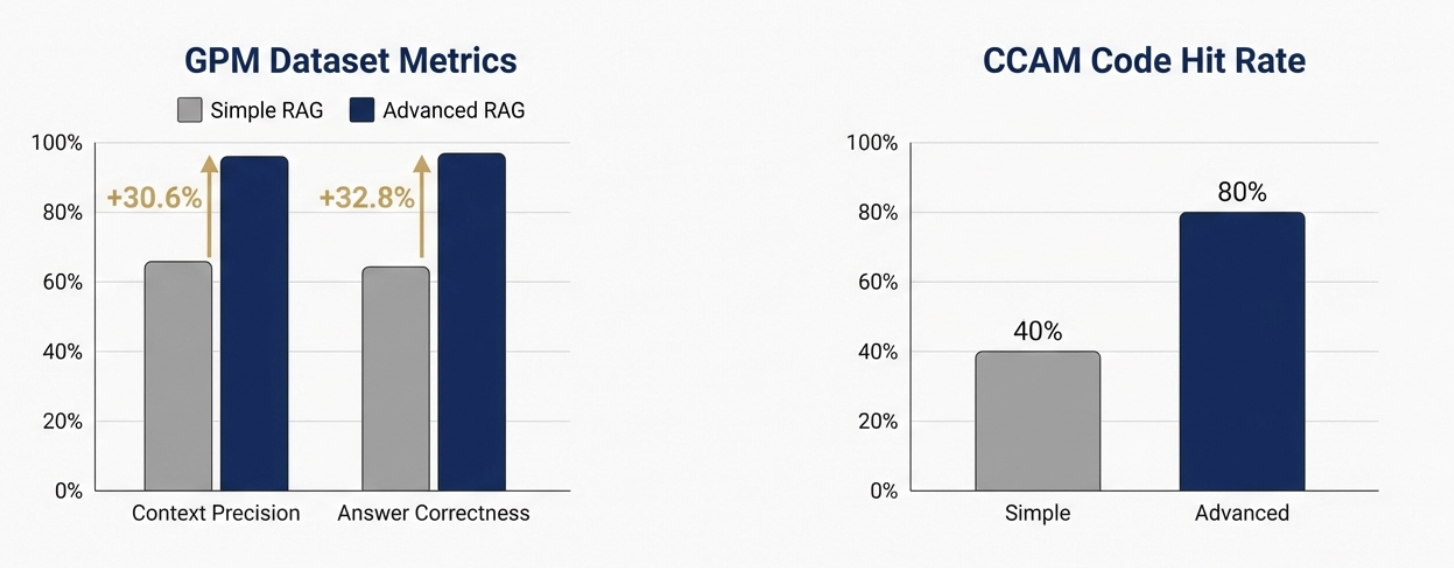
\includegraphics[width=\textwidth]{figures/results_rag.png}
    \end{figure}
\end{frame}

\begin{frame}{Ablation Study: Contribution of Each Component}
    \begin{table}[H]
        \centering
        \caption{Ablation Study on GPM Test Set}
        \begin{tabular}{|l|c|c|c|}
            \hline
            \textbf{Configuration} & \textbf{Precision} & \textbf{$\Delta$ vs Baseline} & \textbf{Cumulative $\Delta$} \\
            \hline
            Baseline (Simple RAG) & 0.648 & --- & --- \\
            \hline
            + UnstructuredIO Parsing & 0.762 & +11.4\% & +11.4\% \\
            \hline
            + Summarization & 0.818 & +5.6\% & +17.0\% \\
            \hline
            + Multilingual E5 Embedding & 0.875 & +5.7\% & +22.7\% \\
            \hline
            + Hybrid Search & 0.92 & +4.5\% & +27.2\% \\
            \hline
            + Reranking & \textbf{0.976} & +5.6\% & \textbf{+32.8\%} \\
            \hline
        \end{tabular}
    \end{table}

\end{frame}



\end{document}